\chapter{Stochastic gradient methods for deep learning}
\section{Gradient Descent}

\begin{prev}
    NN optimization problem:
    \[
        \min_{\bm{\theta}} \; f(\bm{\theta})
    \]
    where \[
        f(\bm{\theta}) = \frac{1}{2C} \bm{\theta}^T \bm{\theta} + \frac{1}{l} \sum_{i=1}^{l} \xi(z^{L+1, i}(\bm{\theta}); \bm{y}^i, \bm{Z}^{1, i})
    \]
    which can be simplify as \[
        f(\bm{\theta}) = \frac{1}{2C} \bm{\theta}^T \bm{\theta} + \frac{1}{l} \sum_{i=1}^{l} \xi(\bm{\theta}; \bm{y}^i, \bm{Z}^{1, i})
    \]
\end{prev}

Now the issue is how to solve this optimization problem, here is a simple method called gradient descent.

\begin{definition}[Gradient Descent]

We let the first order approximation \[
    f(\bm{\theta} + \Delta \bm{\theta}) \approx f(\bm{\theta}) + \nabla f(\bm{\theta})^T \Delta \bm{\theta}
\]
where \[
    \nabla f(\bm{\theta}) = \begin{pmatrix}
        \frac{\partial f(\bm{\theta})}{\partial \bm{\theta}_1} \\
        \vdots \\
        \frac{\partial f(\bm{\theta})}{\partial \bm{\theta}_n}
    \end{pmatrix}
\]

The problem is to solve

    \begin{align*}
        \min_{\Delta \bm{\theta}} \; & \nabla f(\bm{\theta})^T \Delta \bm{\theta} \\
        \text{subject to} \; & \|\Delta \bm{\theta}\| = 1 \tag{2.1}
    \end{align*}

    to find the direction of update $\Delta \bm{\theta}$.
\end{definition}

\begin{note}
    The constraint $\|\Delta \bm{\theta}\| = 1$ is needed to prevent the solution from goes to $-\infty$
\end{note}

\begin{note}
    單變數函數 $f(x)$ 的一階近似為 \[
        f(x + \Delta x) \approx f(x) + f'(x) \Delta x
    \]
    要讓 $f(x + \Delta x)$ 盡可能小,我們需要讓 $f'(x) \Delta x$ 越小越好,因此 $\Delta x$ 的方向應該與 $f'(x)$ 相反,即 $\Delta x = -k f'(x), k > 0$,推到多變數函數上也是一樣的道理,多變數的一階近似是 \begin{align*}
        f(\bm{\theta} + \Delta \bm{\theta}) &\approx f(\bm{\theta}) + \sum_i \left( \frac{\partial f}{\partial \theta_i} \cdot \Delta \theta_i \right) \\
        &= f(\bm{\theta}) + \nabla f(\bm{\theta})^T \Delta \bm{\theta}
    \end{align*}
\end{note}

\begin{theorem}[Gradient Descent Direction]
    The solution of (2.1) is \[
        \Delta \bm{\theta} = - \frac{\nabla f(\bm{\theta})}{\|\nabla f(\bm{\theta})\|} \tag{2.2}
    \]
    , which is called the \textbf{steepest descent direction}(最陡下降方向).
\end{theorem}

However, because we only consider an approximation, which may not strictly decrease the function value, i.e. \[
    f(\bm{\theta}) < f(\bm{\theta} + \Delta \bm{\theta})
\]
might happen. But in general we need the desent property to get convergence, we do the Taylor expansion 
\[
    f(\bm{\theta} + \alpha \Delta \bm{\theta}) = f(\bm{\theta}) + \underbrace{\alpha \nabla f(\bm{\theta})^T \Delta \bm{\theta}}_{\text{critical one while } \alpha \to 0} + \frac{\alpha^2}{2} \Delta \bm{\theta}^T \nabla^2 f(\bm{\theta}) \Delta \bm{\theta} + o(\alpha^2)
\]
where \[
    \nabla^2 f(\bm{\theta}) = \begin{pmatrix}
        \frac{\partial^2 f(\bm{\theta})}{\partial \bm{\theta}_1^2} & \cdots & \frac{\partial^2 f(\bm{\theta})}{\partial \bm{\theta}_1 \partial \bm{\theta}_n} \\
        \vdots & \ddots & \vdots \\
        \frac{\partial^2 f(\bm{\theta})}{\partial \bm{\theta}_n \partial \bm{\theta}_1} & \cdots & \frac{\partial^2 f(\bm{\theta})}{\partial \bm{\theta}_n^2}
    \end{pmatrix}
\]
is the Hessian of $f$ at $\bm{\theta}$.

If \[
    \nabla f(\bm{\theta})^T \Delta \bm{\theta} < 0
\] 
then a small enough $\alpha$ can ensure the descent property (the higher order terms can be ignored). 
\[
    f(\bm{\theta} + \alpha \Delta \bm{\theta}) < f(\bm{\theta})
\]

Thus in the optimization algorithm, it is called a desent direction if it satisfies \[
    \nabla f(\bm{\theta})^T \Delta \bm{\theta} < 0
\]
The direction chose in (2.2) is indeed a descent direction. \[
    -\nabla f(\bm{\theta})^T \frac{\nabla f(\bm{\theta})}{\|\nabla f(\bm{\theta})\|} = - \|\nabla f(\bm{\theta})\| < 0
\]

\subsection{Line Search}

We have known that we have to find a step size $\alpha$ such that \[
    f(\bm{\theta} + \alpha \Delta \bm{\theta}) < f(\bm{\theta})
\]
In optimization, this process is called \textbf{line search}.

\begin{definition}[Exact Line Search] For a one-dimensional optimization problem
    \[
        \min_{\alpha} \; f(\bm{\theta} + \alpha \Delta \bm{\theta})
    \]
\end{definition}

In practice, people usually use \textbf{backtracking line search} or other inexact line search methods to find a suitable step size $\alpha$ with a fixed parameter set $\Delta \bm{\theta}$. We check \[
    \alpha = 1, \beta, \beta^2, \ldots
\]
with $\beta \in (0, 1)$ until \[
    f(\bm{\theta} + \alpha \Delta \bm{\theta}) < f(\bm{\theta}) + \nu \nabla f(\bm{\theta})^T (\alpha \Delta \bm{\theta})
\]
where $\nu \in (0, 1/2)$. 

\begin{definition}[Armijo Condition]
    A step size $\alpha$ is said to satisfy the \textbf{Armijo condition} if
    \[
        f(\bm{\theta} + \alpha \Delta \bm{\theta}) < f(\bm{\theta}) + \nu \nabla f(\bm{\theta})^T (\alpha \Delta \bm{\theta})
    \]
\end{definition}

\begin{note}[Armijo Condition]
    The condition \[
        f(\bm{\theta} + \alpha \Delta \bm{\theta}) < f(\bm{\theta}) + \nu \nabla f(\bm{\theta})^T (\alpha \Delta \bm{\theta})
    \]
    is called the \textbf{Armijo condition}, which is come from the Taylor expansion \begin{align*}
        f(\bm{\theta} + \alpha \Delta \bm{\theta}) &\approx f(\bm{\theta}) + \alpha \nabla f(\bm{\theta})^T \Delta \bm{\theta} \\[3pt]
        \implies f(\bm{\theta} + \alpha \Delta \bm{\theta}) - f(\bm{\theta}) &\approx \alpha \nabla f(\bm{\theta})^T \Delta \bm{\theta} < \nu (\alpha \nabla f(\bm{\theta})^T \Delta \bm{\theta})
    \end{align*}
    Since $\nabla f(\bm{\theta})^T \Delta \bm{\theta} < 0$, we have \[
        \underbrace{\alpha \nabla f(\bm{\theta})^T \Delta \bm{\theta}}_{\text{Directional Derivative of Taylor Expansion's 1st order term}} < \nu (\alpha \nabla f(\bm{\theta})^T \Delta \bm{\theta})
    \]
    Thus the Armijo condition ensures the descent property. 實際下降有到達 $\nu$ 倍的方向導數,就代表這個步長 $\alpha$ 是足夠的.
\end{note}

\vspace{1em}

The convergence of gradient descent with backtracking line search can be guaranteed.

\vspace{1em}

\begin{corollary}
    Every limit point \(\bar{\bm{\theta}}\) of a convergent subsequence of \(\{\bm{\theta}^k\}\) generated by the gradient descent method with backtracking line search, we have \[
        \nabla f(\bar{\bm{\theta}}) = 0
    \]
    which means \(\bar{\bm{\theta}}\) is a stationary point of non-convex problem.
\end{corollary}


\newpage

\subsection{Practical Gradient Descent Algorithm}

It is known that the convergence of gradient descent is slow for difficult problems, thus in practice, method of using \textbf{second-order information} such as Newton's method or Quasi-Newton method are preferred. \[
    f(\bm{\theta} + \Delta \bm{\theta}) \approx f(\bm{\theta}) + \nabla f(\bm{\theta})^T \Delta \bm{\theta} + \frac{1}{2} \Delta \bm{\theta}^T \nabla^2 f(\bm{\theta}) \Delta \bm{\theta}
\]
These methods have faster \textbf{final} convergence rate, below is an illustration of convergence rates.

\begin{figure}[H]
    \centering
    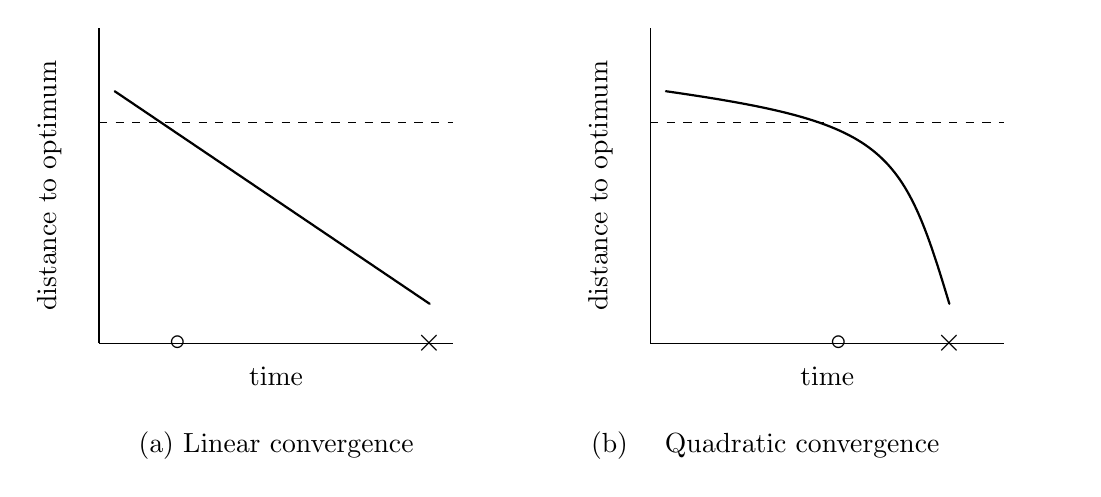
\begin{tikzpicture}[
        % 定義通用樣式
        axis/.style={-}, % 座標軸樣式
        dashed line/.style={dashed, thin}, % 虛線樣式
        curve/.style={thick, line cap=round}, % 曲線樣式
        label text/.style={font=\large}, % 文字大小
        marker/.style={font=\large} % 標記大小
    ]

        % --- 圖 (a): Linear convergence ---
        \begin{scope}
            % 1. 繪製座標軸
            \draw[axis] (0,0) -- (4.5,0) node[midway, below, yshift=-5pt] {time};
            \draw[axis] (0,0) -- (0,4) node[midway, above, rotate=90, yshift=10pt] {distance to optimum};

            % 2. 繪製虛線 (參考線)
            \draw[dashed line] (0,2.8) -- (4.5,2.8);

            % 3. 繪製線性收斂直線
            % 起點 (0.2, 3.2) -> 終點 (4.0, 0.5)
            \draw[curve] (0.2, 3.2) -- (4.2, 0.5);

            % 4. 繪製 x軸上的標記 (圓圈與叉叉)
            \node[marker] at (1.0, 0) {$\circ$}; % 圓圈 (對應圖中位置)
            \node[marker] at (4.2, 0) {$\times$}; % 叉叉 (對應收斂點)

            % 5. 圖說
            \node[below, align=center, text width=5cm] at (2.25, -1) {(a) Linear convergence};
        \end{scope}


        % --- 圖 (b): Superlinear/Quadratic convergence ---
        % 向右平移 7cm
        \begin{scope}[shift={(7,0)}]
            % 1. 繪製座標軸
            \draw[axis] (0,0) -- (4.5,0) node[midway, below, yshift=-5pt] {time};
            \draw[axis] (0,0) -- (0,4) node[midway, above, rotate=90, yshift=10pt] {distance to optimum};

            % 2. 繪製虛線 (參考線)
            \draw[dashed line] (0,2.8) -- (4.5,2.8);

            % 3. 繪製超線性收斂曲線
            % 使用貝茲曲線 (controls) 來模擬前面平緩、後面急遽下降的形狀
            \draw[curve] (0.2, 3.2) .. controls (3.0, 2.8) and (3.2, 2.5) .. (3.8, 0.5);

            % 4. 繪製 x軸上的標記
            \node[marker] at (2.4, 0) {$\circ$}; % 圓圈 (比圖a更靠右)
            \node[marker] at (3.8, 0) {$\times$}; % 叉叉

            % 5. 圖說
            \node[below, align=left, text width=6cm] at (2.25, -1) {(b) \quad Quadratic convergence};
        \end{scope}

    \end{tikzpicture}
    \caption{Convergence Rates of Different Methods}
\end{figure}

But in deep learning, fast final convergence may not be that important, since the optimal solution $\bm{\theta}^*$ is not necessarily the best generalization solution.

\section{Stochastic Gradient Method}

\subsection{Estimation of Gradient}

\begin{prev}
    The objective function is \[
        f(\bm{\theta}) = \frac{1}{2C} \bm{\theta}^T \bm{\theta} + \frac{1}{l} \sum_{i=1}^{l} \xi(\bm{\theta}; \bm{y}^i, \bm{Z}^{1, i})
    \]
    The gradient is \[
        \frac{\bm{\theta}}{C} + \frac{1}{l} \nabla_{\bm{\theta}} \left( \sum_{i=1}^{l} \xi(\bm{\theta}; \bm{y}^i, \bm{Z}^{1, i}) \right) = \frac{\bm{\theta}}{C} + \frac{1}{l} \sum_{i=1}^{l} \nabla_{\bm{\theta}} \xi(\bm{\theta}; \bm{y}^i, \bm{Z}^{1, i})
    \]
    \begin{note}
        $\nabla_{\bm{\theta}}$ denotes the gradient with respect to $\bm{\theta}$, which is used to compute the gradient of function $\xi$ only.
    \end{note}
\end{prev}

Going over all data is time-consuming, thus if data are from same distribution \[
    \mathbb{E}(\nabla_{\bm{\theta}} \xi(\bm{\theta}; \bm{y}^i, \bm{Z}^{1})) = \frac{1}{l} \sum_{i=1}^{l} \nabla_{\bm{\theta}} \xi(\bm{\theta}; \bm{y}^i, \bm{Z}^{1, i})
\]
then we can just use a \textbf{subset} of data $S$, which is often called a \textbf{batch}, to estimate the gradient \[
    \frac{\bm{\theta}}{C} + \frac{1}{|S|} \sum_{i: i \in S} \nabla_{\bm{\theta}} \xi(\bm{\theta}; \bm{y}^i, \bm{Z}^{1, i})
\]

\newpage

With the estimated gradient, and the for $\eta$ is the \textbf{learning rate} or \textbf{step size}, which is hard to choose in practice. We can get the \textbf{stochastic gradient algorithm} as below.

\SetAlgoNoLine
\DontPrintSemicolon

\begin{algorithm}
    \caption{Stochastic Gradient Algorithm}
    Given an initial learning rate $\eta$.\;
    
    \While{}{
        Choose $S \subset \{1, \dots, l\}$.\;
        
        Calculate
        \[
            \boldsymbol{\theta} \leftarrow \boldsymbol{\theta} - \eta \left( \frac{\boldsymbol{\theta}}{C} + \frac{1}{|S|} \nabla_{\boldsymbol{\theta}} \sum_{i: i \in S} \xi(\boldsymbol{\theta}; \boldsymbol{y}^i, Z^{1,i}) \right)
        \]
        
        % 行號 5
        May adjust the learning rate $\eta$\;
    }
\end{algorithm}

By the name of stochastic gradient, we know that the gradient used here is a random estimation of the true gradient. Compared to the true gradient, this method does not do ``searching'' for a good step size $\alpha$. Without the full gradient information, the decrease condition such as Armijo condition cannot be guaranteed. Thus, we don't have an algorithm with ``decent'' property, i.e. it is possible for \[
    f(\bm{\theta}^{\text{next}}) > f(\bm{\theta})
\]

\subsection{Momentum Method}

To improve the convergence speed of stochastic gradient method, we can use the \textbf{momentum method}.

\begin{definition}[Momentum Method]\label{def:momentum_method}
    Let $\bm{v}$ be the velocity vector, initialized as $\bm{v} = 0$. The momentum method updates $\bm{\theta}$ as follows: 
    \begin{align*}
        \bm{v} &\leftarrow \alpha \bm{v} - \eta \left( \frac{\bm{\theta}}{C} + \frac{1}{|S|} \nabla_{\bm{\theta}} \sum_{i: i \in S} \xi(\bm{\theta}; \bm{y}^i, \bm{Z}^{1, i}) \right) \\[3pt]
        \bm{\theta} &\leftarrow \bm{\theta} + \bm{v}
    \end{align*}
    with $\alpha \in [0, 1)$ being the momentum parameter.
\end{definition}

In this method, we use the previous gradient information to smooth the update direction. We use exponential moving average to compute the $\bm{\theta}$, i.e expend the recurrence:
\begin{align*}
    \bm{\theta} \leftarrow \bm{\theta} &- \eta\ (\text{current sub-gradient}) \\
    &- \alpha \eta\ (\text{previous sub-gradient}) \\
    &- \alpha^2 \eta\ (\text{sub-gradient before previous})
\end{align*}
The effect of the sub-gradient from earlier iterations decays exponentially with factor $\alpha \in [0, 1)$. The data we select in each iteration is to approximate the true gradient, thus the resulting update direction is noisy. By using momentum (averaging), we can reduce the variance of the update direction, thus the convergence speed is improved. However, the rule of Definition~\ref{def:momentum_method} might be biased since the initial velocity, which will disscussed in later lectures.

\newpage

\subsection{AdaGrad (Adaptive Gradient Algorithm)}

\begin{quotation}
    Scaling learning rates inversely proportional to the \textbf{square root of sum of past gradient squares}. (Duchi et al., 2011)
\end{quotation}

The idea of AdaGrad is to adapt the learning rate for each parameter according to the historical gradient information.

\begin{notation}[$\odot$]
    For two vectors $\bm{a}, \bm{b} \in \mathbb{R}^n$, the \textbf{Hadamard product} (element-wise product) is defined as \[
        \bm{a} \odot \bm{b} = \begin{pmatrix}
            a_1 b_1 \\
            a_2 b_2 \\
            \vdots \\
            a_n b_n
        \end{pmatrix}
    \]
\end{notation}

\begin{definition}[AdaGrad]
    Let $\bm{g}$ be the stochastic gradient, $\bm{r}$ be the adjusted gradient. AdaGrad updates $\bm{\theta}$ as follows:
    \begin{align*}
        \bm{g} &\leftarrow \frac{\bm{\theta}}{C} + \frac{1}{|S|} \nabla_{\bm{\theta}} \sum_{i: i \in S} \xi(\bm{\theta}; \bm{y}^i, \bm{Z}^{1, i}) \\[3pt]
        \bm{r} &\leftarrow \bm{r} + \bm{g} \odot \bm{g} \\[3pt]
        \bm{\theta} &\leftarrow \bm{\theta} - \frac{\epsilon}{\sqrt{\bm{r}} + \delta} \odot \bm{g}
    \end{align*}
    where $\epsilon, \delta$ are hyperparameters and $\bm{r}$ is the accumulated squared gradient.
\end{definition}

The learning rate for each parameter is scaled by $\frac{1}{\bm{r}}$, which means that if a parameter has a large historical gradient, its learning rate will be reduced, and vice versa. 

\begin{note}
    Square is used to ensure all movements of parameters not be canceled out. $\delta$ is used to prevent division by zero.
\end{note}

For this computation, we can let the frequently updated parameters have smaller learning rates, while the infrequently updated parameters have larger learning rates, which is to let learner take notice on those infrequently features.

\begin{recall}
    In linear classification problem, the optimization problem is \[
        \frac{\bm{w}^T \bm{w}}{2} + C \sum_{i=1}^{l} \xi(\bm{w}; \bm{x}_i, y_i)
    \]
\end{recall}

For method like SVM or logistic regression, the loss function can be written as a function of $\bm{w}^T \bm{x}$. \[
    \xi(\bm{w}; y, \bm{x}) = \hat{\epsilon}(\bm{w}^T \bm{x})
\]
Then the gradient is \[
    \nabla_{\bm{w}} \xi(\bm{w}; y, \bm{x}) = \bm{w} + C \sum_{i=1}^{l} \hat{\epsilon}'(\bm{w}^T \bm{x}_i) \bm{x}_i
\]
The expression shows that \[
    \nabla \bm{w} = \bm{w} + C \sum (\text{error}) \cdot \mathbf{x}_i
\]
which indicates that the gradient is affected by the \textbf{density} of features.

However, the above analysis is not suitable for ``non-convex'' case such as neural networks. Empirically, AdaGrad will meet the problem of ``too fast decay of learning rate'', thus other adaptive methods such as RMSProp or Adam are proposed to solve this problem.

\subsection{RMSProp (Relative Mean Square Propagation)}

For convex problems, such as SVM or logistic regression, AdaGrad works well since the objective function is convex. However, for non-convex problems such as neural networks, AdaGrad's learning rate may be too small before reaching the convex region, i.e. $\bm{r}$ becomes too large while not reaching the optimal solution in the non-convex case. Thus, RMSProp is proposed to solve this problem, which uses \red{\textbf{exponential weighted moving average}} to compute the accumulated squared gradient.

\begin{definition}[RMSProp]
    Let $\bm{g}$ be the stochastic gradient, $\bm{r}$ be the adjusted gradient. RMSProp updates $\bm{\theta}$ as follows:
    \begin{align*}
        \bm{g} &\leftarrow \frac{\bm{\theta}}{C} + \frac{1}{|S|} \nabla_{\bm{\theta}} \sum_{i: i \in S} \xi(\bm{\theta}; \bm{y}^i, \bm{Z}^{1, i}) \\[3pt]
        \bm{r} &\leftarrow \rho \bm{r} + (1 - \rho) (\bm{g} \odot \bm{g}) \\[3pt]
        \bm{\theta} &\leftarrow \bm{\theta} - \frac{\epsilon}{\sqrt{\bm{r}} + \delta} \odot \bm{g}
    \end{align*}
    where $\epsilon, \delta$ are hyperparameters, $\rho \in [0, 1)$ is the decay rate, and $\bm{r}$ is the exponentially weighted moving average of squared gradients.
\end{definition}

However, RMSProp is somehow heuristic compared to AdaGrad, since there is no theoretical guarantee for its convergence.

\subsection{Adam (Adaptive Moment Estimation)}

\begin{definition}[Adam]
    Let $\bm{g}$ be the stochastic gradient, $\bm{s}$ be the first moment vector, $\bm{r}$ be the second moment vector. Adam updates $\bm{\theta}$ as follows:
    \begin{align*}
        \bm{g} &\leftarrow \frac{\bm{\theta}}{C} + \frac{1}{|S|} \nabla_{\bm{\theta}} \sum_{i: i \in S} \xi(\bm{\theta}; \bm{y}^i, \bm{Z}^{1, i}) \\[3pt]
        \bm{s} &\leftarrow \rho_1 \bm{s} + (1 - \rho_1) \bm{g} \\[3pt]
        \bm{r} &\leftarrow \rho_2 \bm{r} + (1 - \rho_2) (\bm{g} \odot \bm{g}) \\[3pt]
        \hat{\bm{s}} &\leftarrow \frac{\bm{s}}{1 - \rho_1^t} \\[3pt]
        \hat{\bm{r}} &\leftarrow \frac{\bm{r}}{1 - \rho_2^t} \\[3pt]
        \bm{\theta} &\leftarrow \bm{\theta} - \frac{\epsilon}{\sqrt{\hat{\bm{r}}} + \delta} \odot \hat{\bm{s}}
    \end{align*}
    where $t$ is the iteration number.
\end{definition}

Roughly speaking, Adam combines the ideas of momentum method and RMSProp. But the use of \[
    \frac{\epsilon}{\sqrt{\hat{\bm{r}}} + \delta} \odot \hat{\bm{s}}
\]
is somewhat heuristic, and there is no theoretical guarantee for better convergence. However, Adam works fairly robust to the choice of hyperparameters in practice. However, recent research shows that Adam actually find worse solutions than SGD in some cases.

Now we consider \begin{align*}
    \hat{\bm{s}} &\leftarrow \frac{\bm{s}}{1 - \rho_1^t} \\[3pt]
    \hat{\bm{r}} &\leftarrow \frac{\bm{r}}{1 - \rho_2^t}
\end{align*}
which are called ``\textbf{bias correction}''.\\

Note that we use $\bm{s}$ as the direction of update $\bm{\theta}$. We hope that its expectation is similar to the expected gradient, i.e. \[
    \begin{cases}
        \mathbb{E}[\bm{s}_t] = \mathbb{E}[\bm{g}_t] \\[3pt]
        \mathbb{E}[\bm{r}_t] = \mathbb{E}[\bm{g}_t \odot \bm{g}_t]
    \end{cases}
\]
where $t$ is the iteration number. However, since $\bm{s}$ and $\bm{r}$ are affected a lot by the initial value by the moving average, i.e. the vector is biased towards the initial value (which is $\bm{0}$). 

\begin{theorem}
    The bias correction of $\bm{s}_t$ is \[
        \hat{\bm{s}} \leftarrow \frac{\bm{s}}{1 - \rho_1^t}
    \]
\end{theorem}
\begin{proof}
    For $\bm{s}_t$ we have \begin{align*}
        \bm{s}_t &= \rho_1 \bm{s}_{t-1} + (1 - \rho_1) \bm{g}_t \\[3pt]
        &= \rho_1(\rho_1 \bm{s}_{t-2} + (1 - \rho_1) \bm{g}_{t-1}) + (1 - \rho_1) \bm{g}_t \\[3pt]
        &= (1 - \rho_1) \sum_{i=1}^{t} \rho_1^{t-i} \bm{g}_i
    \end{align*}
    
    Then, \[
        \mathbb{E}[\bm{s}_t] = \mathbb{E}\left[ (1 - \rho_1) \sum_{i=1}^{t} \rho_1^{t-i} \bm{g}_i \right] = \mathbb{E}[\bm{g}_i] \cdot (1 - \rho_1) \sum_{i=1}^{t} \rho_1^{t-i}
    \]

    Note that we assume \[
        \mathbb{E}[\bm{g}_i] = \mathbb{E}[\bm{g}_t], \forall i \leq t
    \]

    Thus, \[
        (1-\rho_1) \sum_{i=1}^{t} \rho_1^{t-i} = (1 - \rho_1) (1 + \rho_1 + \rho_1^2 + \cdots + \rho_1^{t-1}) = 1 - \rho_1^t
    \]

    Hence, \[
        \mathbb{E}[\bm{s}_t] = (1 - \rho_1^t) \mathbb{E}[\bm{g}_t]
    \]

    Therefore, to correct the bias, we have \[
        \hat{\bm{s}}_t = \frac{\bm{s}_t}{1 - \rho_1^t} \ \implies \ \mathbb{E}[\hat{\bm{s}}_t] = \mathbb{E}[\bm{g}_t]
    \]
\end{proof}

Use the same idea, we can prove the bias correction of $\bm{r}_t$.

\newpage

\begin{theorem}
    The bias correction of $\bm{r}_t$ is \[
        \hat{\bm{r}} \leftarrow \frac{\bm{r}}{1 - \rho_2^t}
    \]
\end{theorem}
\begin{proof}
    For $\bm{r}_t$ we have \begin{align*}
        \bm{r}_t &= \rho_2 \bm{r}_{t-1} + (1 - \rho_2) (\bm{g}_t \odot \bm{g}_t) \\[3pt]
        &= \rho_2(\rho_2 \bm{r}_{t-2} + (1 - \rho_2) (\bm{g}_{t-1} \odot \bm{g}_{t-1})) + (1 - \rho_2) (\bm{g}_t \odot \bm{g}_t) \\[3pt]
        &= (1 - \rho_2) \sum_{i=1}^{t} \rho_2^{t-i} (\bm{g}_i \odot \bm{g}_i)
    \end{align*}
    
    Then, \[
        \mathbb{E}[\bm{r}_t] = \mathbb{E}\left[ (1 - \rho_2) \sum_{i=1}^{t} \rho_2^{t-i} (\bm{g}_i \odot \bm{g}_i) \right] = \mathbb{E}[\bm{g}_i \odot \bm{g}_i] \cdot (1 - \rho_2) \sum_{i=1}^{t} \rho_2^{t-i}
    \]

    Note that we assume \[
        \mathbb{E}[\bm{g}_i \odot \bm{g}_i] = \mathbb{E}[\bm{g}_t \odot \bm{g}_t], \forall i \leq t
    \]

    Thus, \[
        (1-\rho_2) \sum_{i=1}^{t} \rho_2^{t-i} = (1 - \rho_2) (1 + \rho_2 + \rho_2^2 + \cdots + \rho_2^{t-1}) = 1 - \rho_2^t
    \]

    Hence, \[
        \mathbb{E}[\bm{r}_t] = (1 - \rho_2^t) \mathbb{E}[\bm{g}_t \odot \bm{g}_t]
    \]
\end{proof}

Here is an interesting story about BERT, which is an important NLP technique using Adam as the optimizer. The original BERT forget to use bias correction, which seems to cause lengthy training iterations.

\subsection{AdamW (Adam with Weight Decay)}

Now we consider the weight decay term,
\begin{recall}
    The update of stochastic gradient method is \[
        \boldsymbol{\theta} \leftarrow \boldsymbol{\theta} - \eta \left( \frac{\boldsymbol{\theta}}{C} + \frac{1}{|S|} \nabla_{\boldsymbol{\theta}} \sum_{i: i \in S} \xi(\boldsymbol{\theta}; \boldsymbol{y}^i, Z^{1,i}) \right)
    \]
\end{recall}

In this case, \[
    \frac{\boldsymbol{\theta}}{C}
\]
come from the regularization term \(\bm{\theta}^T \bm{\theta}/2\) in $f(\bm{\theta})$. However, in neural networks, people usually use \textbf{weight decay} to replace the regularization term, which is implemented as \[
    \bm{\theta} \leftarrow (1 - \lambda) \bm{\theta} - \eta \left( \frac{1}{|S|} \nabla_{\bm{\theta}} \sum_{i: i \in S} \xi(\bm{\theta}; \bm{y}^i, \bm{Z}^{1, i}) \right)
\]
where $\lambda$ is the rate of weight decay factor. There is no  a theoretical reason for this modification. But clearly, if \[
    \lambda = \frac{\eta}{C}
\]
then weight decay is equivalent to the regularization. However, if using adaptive methods such as Adam, the equivalence does not hold. For instance, in AdaGrad, the update is 
\[
    \bm{\theta} \leftarrow \bm{\theta} - \frac{\epsilon}{\sqrt{\bm{r}} + \delta} \odot \left( \frac{1}{|S|} \nabla_{\bm{\theta}} \sum_{i: i \in S} \xi(\bm{\theta}; \bm{y}^i, \bm{Z}^{1, i}) \right) - \frac{\epsilon}{\sqrt{\bm{r}} + \delta} \odot \frac{\bm{\theta}}{C}
\]
so the regularization term is scaled in a component-wise way. Hence, we try to decouple the weight decay step from the gradient step. For example, for momentum method \begin{align*}
    \bm{v} &\leftarrow \alpha \bm{v} - \eta \left( \frac{\bm{\theta}}{C} + \frac{1}{|S|} \nabla_{\bm{\theta}} \sum_{i: i \in S} \xi(\bm{\theta}; \bm{y}^i, \bm{Z}^{1, i}) \right) \\[3pt]
    \bm{\theta} &\leftarrow \bm{\theta} + \bm{v}
\end{align*}
we use weight decay as the equivalence \begin{align*}
    \bm{v} &\leftarrow \alpha \bm{v} - \eta \left( \frac{1}{|S|} \nabla_{\bm{\theta}} \sum_{i: i \in S} \xi(\bm{\theta}; \bm{y}^i, \bm{Z}^{1, i}) \right) \\[3pt]
    \bm{\theta} &\leftarrow \bm{\theta} + \bm{v} - \red{\eta \frac{\bm{\theta}}{C}}
\end{align*}

This modification is called AdamW when using Adam as the optimizer.

\begin{definition}[AdamW]
    Let $\bm{g}$ be the stochastic gradient, $\bm{s}$ be the first moment vector, $\bm{r}$ be the second moment vector. AdamW updates $\bm{\theta}$ as follows:
    \begin{align*}
        \bm{g} &\leftarrow \frac{1}{|S|} \nabla_{\bm{\theta}} \sum_{i: i \in S} \xi(\bm{\theta}; \bm{y}^i, \bm{Z}^{1, i}) \\[3pt]
        \bm{s} &\leftarrow \rho_1 \bm{s} + (1 - \rho_1) \bm{g} \\[3pt]
        \bm{r} &\leftarrow \rho_2 \bm{r} + (1 - \rho_2) (\bm{g} \odot \bm{g}) \\[3pt]
        \hat{\bm{s}} &\leftarrow \frac{\bm{s}}{1 - \rho_1^t} \\[3pt]
        \hat{\bm{r}} &\leftarrow \frac{\bm{r}}{1 - \rho_2^t} \\[3pt]
        \bm{\theta} &\leftarrow \bm{\theta} - \frac{\epsilon}{\sqrt{\hat{\bm{r}}} + \delta} \odot \hat{\bm{s}} - \red{\epsilon \frac{\bm{\theta}}{C}}
    \end{align*}
\end{definition}

AdamW is not equivalent to Adam with $\bm{\theta}/C$ is added after the gradient calculation. There is the disscussion about why AdamW works better than Adam in practice in the paper \href{https://arxiv.org/abs/1711.05101}{Decoupled Weight Decay Regularization}.

\subsection{Why Stochastic Gradient?}

We can simply conclude four reasons to use stochastic gradient methods in practice.
\begin{enumerate}[label=$\arabic*^\circ$]
    \item \textbf{Final convergence is not important.} In deep learning, the optimal solution $\bm{\theta}^*$ may not lead to the best model. Futher, we don't need to reach the optimal solution, instead, we find \[
        \arg \max_{k} z_k^{L+1}(\bm{\theta})
    \] 
    , so not-so-accurate solution is acceptable.
    \item \textbf{Cheap iterations.} There is a property for data classification in statistics \[
        \mathbb{E}[\nabla_{\bm{\theta}} \xi(\bm{\theta}; \bm{y}^i, \bm{Z}^{1, i})] = \frac{1}{l} \nabla_{\bm{\theta}} \sum_{i=1}^{l} \xi(\bm{\theta}; \bm{y}^i, \bm{Z}^{1, i})
    \]
    thus, we can cheaply estimate the gradient by using a subset of data. Indeed, stochastic gradient is less used outside deep learning.

    \begin{remark}
        Nowadays, in complicated models we stochastic gradient is simpler than calculating the full gradient with Hessian. Gradient calculation of stochastic gradient can be easily implemented by \textbf{automatic differentiation} which will discussed later.
    \end{remark}
    
    \item \textbf{Non-convex problems.} For convex problems, second-order methods such as Newton's method or Quasi-Newton method are preferred since they find global optimal solutions more efficiently. However, for non-convex problems such as neural networks, efficiency to find stationary points is less important since local optimal solutions may generalize better.
\end{enumerate}

All these are the reasons why stochastic gradient methods are widely used in deep learning.